\chapter[Introdução]{Introdução}

O aumento da capacidade de armazenamento e processamento de dados tem possibilitado o desenvolvimento de sistemas inteligentes através do aprendizado de máquina. Tal desenvolvimento, por sua vez, permitiu avanços em diversas áreas da computação, microeletrônica e sensoriamento. 

Hoje, aplicações tais como pesquisas web, sistemas \textit{anti-spam}, reconhecimento de voz, recomendações de produto e diversas outras são frutos desse progresso. Porém a disponibilidade de quantidades massivas de dados, apresenta não só um horizonte vasto de possíveis aplicações, mas também desafios para seleção e processamento desses dados.


\section{Aprendizado de Máquina}

Aprendizado de máquina é o campo da computação responsável por desenvolver e empregar sistemas ou modelos que, através da sua exposição à experiências, são capazes de melhorar sua performance na realização de determinada tarefa \cite{mitchell_1997}.

O processo de desenvolvimento de modelos com aprendizado de máquina pode ser dividido, em linhas gerais, em duas grandes etapas. A primeira delas refere-se à análise e tratamento dos dados. Nessa etapa procura-se identificar correlações entre as informações disponíveis e as variáveis de interesse. Além disso, são explorados possíveis filtros, transformações e outros algoritmos que possam facilitar o aprendizado do modelo. Também é necessário realizar nessa etapa a separação dos dados que serão utilizados para treinamento, validação e teste no decorrer do processo.

\begin{figure}[!htb]
    \caption{Fluxo geral de desenvolvimento de sistemas de aprendizado de máquina.}
    \begin{center}
    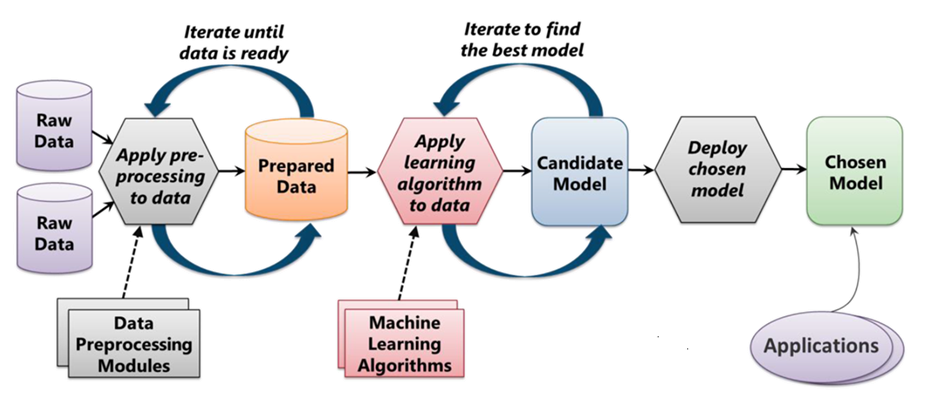
\includegraphics[width=\linewidth]{imgs/intro/MLFlow}
    \end{center}
    \legend{Fonte: \textit{Machine Learning: A Gentle Introduction \cite{mlflow}}. Adaptado.}
    \label{fig:mlflow}
\end{figure}

Na etapa seguinte objetiva-se obter um modelo capaz de reproduzir o comportamento do sistema que gerou o conjunto de dados. Para tal, um ou mais modelos e algoritmos são selecionados e treinados. Duas características são de fundamental importância e devem ser controladas: a capacidade de representação do sistema (complexidade) e a capacidade de extrapolação das saídas para novas entradas (generalização).

Os algoritmos utilizados nesta segunda etapa podem ser classificados em uma de três categorias, de acordo com as características dos dados disponíveis. \cite{ai_modern}

Na categoria de aprendizado não supervisionado, desenvolve-se sistemas capazes identificar padrões implícitos em um conjunto de dados não rotulados.

No aprendizado por reforço, os sistemas se adaptam de acordo com dados de resposta oriundos do ambiente no qual estão envolvidos.

Por fim, no aprendizado supervisionado, estão modelos que, a partir de um conjunto de entradas e saídas conhecidas, são capazes de extrapolar a dinâmica do sistema em questão.

\section{Generalização e Complexidade}

O processo de aprendizado supervisionado é a inferência de um mapeamento de dados de entrada a variáveis de saída a partir de um conjunto de observações. Este pode, portanto, ser interpretado como um ajuste, linear ou não, de uma curva \cite{haykin}. Consequentemente, os modelos obtidos através desse processo também estão sujeitos a \textit{overfitting} e \textit{underfitting}.

\textit{Overfitting}, ou sobre-ajuste, é caracterizado pela alta performance no conjunto de dados de treinamento e baixa performance em dados nunca observados. Isto é, o modelo assimila desvios causados por erros de medição ou fatores aleatórios presentes no treinamento. Dessa maneira, o erro em relação aos dados de treinamento é reduzido, porém essa melhora não corresponde a uma melhora na representação da realidade.

De maneira similar, o \textit{underfitting},ou sub-ajuste, é caracterizado pela baixa performance em ambos os conjuntos de dados, indicando que o modelo utilizado não é capaz de representar de maneira satisfatória a complexidade do sistema real.

\begin{figure}[H]
    \caption{Relação entre underfitting-overfitting, generalização-complexidade e viés-variância.}
    \begin{center}
    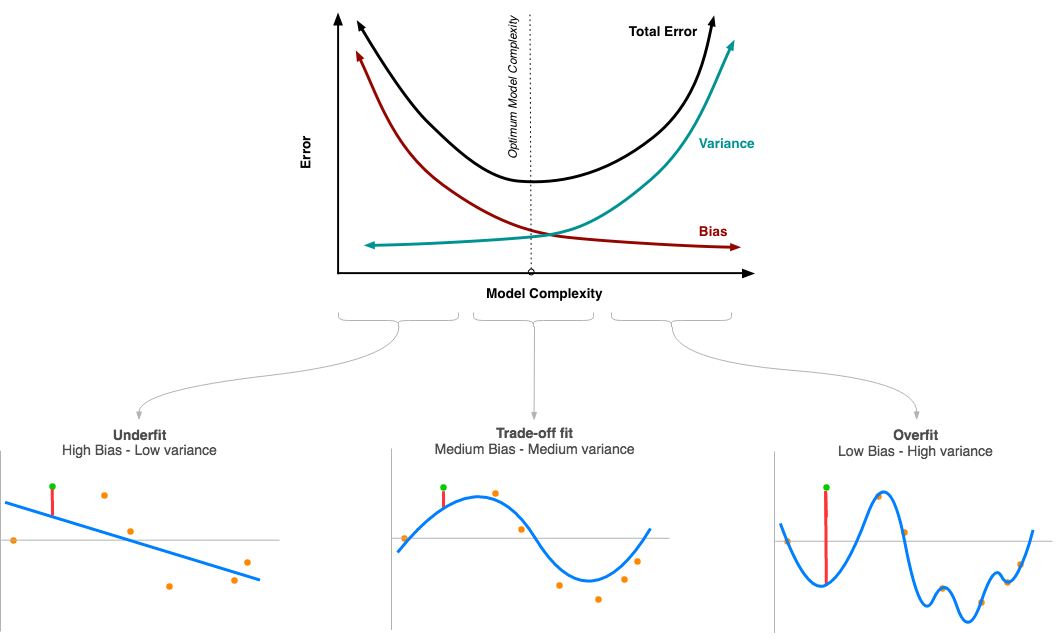
\includegraphics[width=\linewidth]{imgs/intro/over_underfitting}
    \end{center}
    \legend{Fonte: \textit{Bias and Variance} \cite{bias_var}. Adaptado.}
    \label{fig:over_underfitting}
\end{figure}

Generalização é o termo usado para descrever a capacidade de um sistema de reagir de maneira satisfatória a novos dados. Isto é, após realizado o treinamento, a capacidade de um sistema de realizar predições precisas (sem \textit{overfitting} ou \textit{underfitting}) para dados nunca observados.

Analogamente, pode-se avaliar o modelo em termos de complexidade, onde modelos mais complexos são capazes de ajustar os dados em uma família maior de curvas, porém estão mais sujeitos a \textit{overfitting} e exigem, em geral uma complexidade amostral (\textit{sample complexity}) maior.

Pode-se ainda avaliar o sistema em termos de viés e variância (\textit{bias-variance tradeoff}), onde o viés representa a parcela do erro atribuída à diferença entre o modelo e a função real do sistema, e a variância a parcela devido à sensibilidade do modelo à pequenas variações nos dados.

\section{O problema da dimensionalidade}

Sistemas que se utilizam de aprendizado de máquina apresentam respostas baseados nos dados de entrada que lhe são apresentados. Dessa maneira, a determinação de que variáveis são relevantes para o sistema é uma etapa fundamental de seu processo de desenvolvimento.

A inclusão de variáveis irrelevantes resulta no aumento da complexidade do modelo, o tornando mais suscetível ao \textit{overfitting} e menos interpretável \cite[p. 204]{intro_stat_learn}. Além disso, um número elevado de variáveis de entrada resulta em um efeito conhecido como a maldição da dimensionalidade (\textit{curse of dimensionality}), onde o aumento do número de dimensões (quantidade de variáveis), implica no aumento exponencial do número de amostras necessárias para representar o espaço de variáveis \cite[p. 34]{bishop_2006}.

\begin{figure}[!htb]
    \caption{Crescimento do espaço de variáveis em virtude do aumento das dimensões.}
    \begin{center}    
    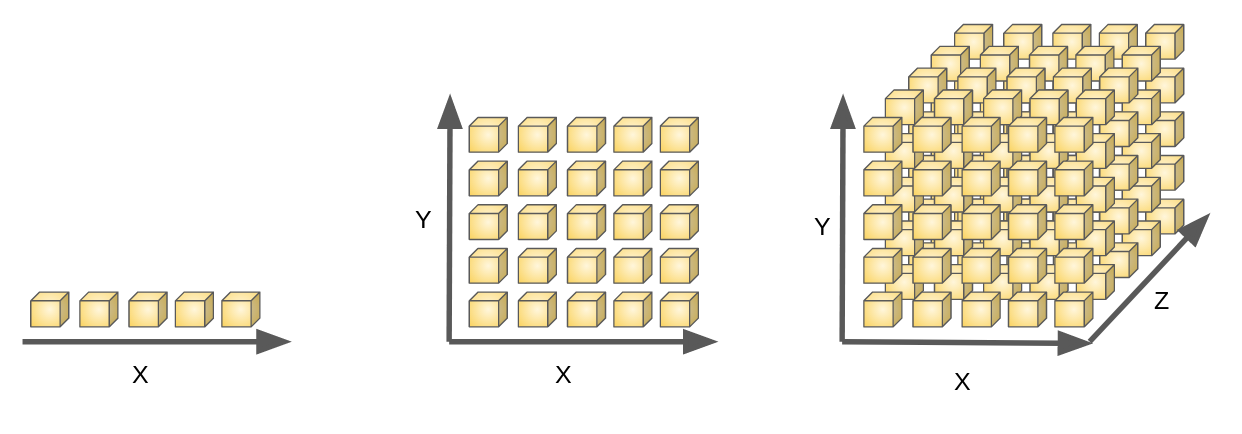
\includegraphics[width=0.8\textwidth]{imgs/rev/dimensionalty_grown.png}
    \end{center}
    \legend{Fonte: The Curse of Dimensionality \cite{dim_grown}}
    \label{fig:dim_grown}
\end{figure}

\begin{figure}[!htb]
    \caption{Performance em relação ao número de dimensões e amostras.}
    \begin{center}  
    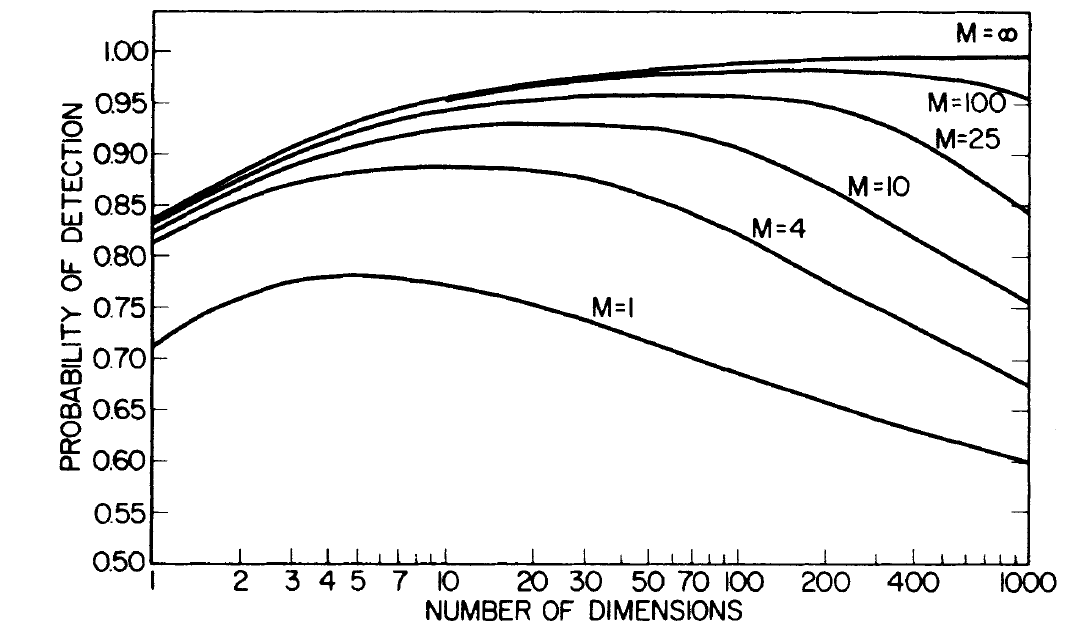
\includegraphics[width=0.5\textwidth]{imgs/rev/dim_performance}
    \end{center}
    \legend{Fonte: A Problem of Dimensionality: A Simple Example \cite{art:prob_dim}}
    \label{fig:dim_perf}
\end{figure}

É desejável então que se utilize o menor número possível de variáveis de entrada que permitam ao modelo produzir a resposta correta. Uma maneira de realizar essa redução de dimensionalidade é selecionar um subconjunto das variáveis disponíveis, descartando aquelas que apresentarem pouca ou nenhuma relevância para o problema \cite[p. 204]{intro_stat_learn}.


\section{Motivação}
A quantidade e qualidade das variáveis incluídas em um modelo é responsável por parcela significativa de sua complexidade e potencial de generalização. Para o desenvolvimento de um modelo satisfatório, é necessário, portanto, a aplicação de procedimentos adequados para a seleção e processamento dos dados iniciais.

Esse trabalho apresenta um método de seleção automática de variáveis de entrada para modelos treinados através de aprendizado supervisionado.

\section{Objetivos}

 O algoritmo desenvolvido visa a obtenção de um conjunto de variáveis que possa ser usado para o treinamento de modelos com alta capacidade de generalização. 
 
 É um método de seleção de variáveis \textit{stepwise} e, portanto, realiza uma busca gananciosa (\textit{greedy search}) em um conjunto de variáveis candidatas, selecionando, a cada iteração, a variável que apresentar a maior melhora na performance, segundo a métrica adotada.
 
Nesse trabalho, faz-se o uso de um modelo de baixa complexidade (regressão linear regularizada), aliado ao erro de validação cruzada \textit{leave-one-out}, para se determinar a variação da performance ao se incluir uma variável.